% kelompok 2 TUGAS 3 GIS (Database Acces)
%Tiara Rizki Wulansari (1154026)
%Mohammad Agung Deomartha (1154032)

\section{Sending Email}
	Mail Server adalah perangkat lunak program yang mendistribusikan file atau informasi sebagai respons atas permintaan yang dikirim via email, mail server juga digunakanpadabitnetuntukmenyediakanlayananserupaftp. Selainitumailserverjuga dapat dikatakan sebagai aplikasi yang digunakan untuk penginstalan email.	\par \vspace{12pt}
	Tak hanya sebagai sebuah program mail server juga bisa berupa sebuah komputer yang memang dikhususkan untuk menjalankan sebuah aplikasi perangkat lunak program ini. nah komputer ini di ibaratkan sebagai jantung dari system sebuah email. Program ini biasanya dikelola oleh programer yang disebut dengan post master.	\par \vspace{12pt}
	Mail server ini dikelola oleh seorang post master yang memiliki beberapa tugas pokok yaitu mengelola kaun, memonitor bagaimana kinerja server dan melaksanakan tugas administrative lainnya. Biasanya program ini menggunakan protocol antara lain smtp, pop3 dan imap.	\par \vspace{12pt}
	
	\textbf{Cara Kerja Mail Server}	\par \vspace{12pt}
	
	Setelah kamu tahu apa itu mail server, kini saatnya kamu tahu bagaimana mail server bekerja. Pada dasarnya ada dua cara kerja program ini. pertama, proses pengiriman email akan melewati tahapan yang agak panjang. saat email dikirim karena email akan disimpan pada server utama atau email server itu sendiri berdasarkan tujuan email akan dikirimkan kemana. Umumnya file ini berisi informasi yang dimana sumber tujuan, serta adanya waktu pengiriman. Nah saat kamu sebagai user membaca email berarti user telah mengakses server email tersebut dan membaca email yang tersimpan pada server yang di tampilkan pada browser pengguna.	\par \vspace{12pt}
	
	Untuk memahami cara kerja mail server yang kedua ini,kamu harus memahami ada beberapa istilah penting yaitu MUA atau mail user agent yaitu sebuah komponen yang berinteraksi secara langsung, misalnya adalah thunderbird, ms outlook, zimbra atau interface webmail seperti gmail ataupun yahoo.	\par \vspace{12pt}
	
	Selain itu istilah penting mail server lainnya adalah MTA atau mail transfer agent yang bertanggung jawab mentransfer email dari server mail kemudian sampai server mail penerima, contohnya adalah karena sendmail dan postfix. Selain itu MDA atau mail delivery agent, jika mta lokasi menerima email masuk dari mta terpencil maka email akan dikirim kek otak pengguna dengan mda.	\par \vspace{12pt}
	
	Istilah lain dalam mail server ada POP atau IMAP kedua singkatan ini merupakan sesuatu protocol yang digunakan untuk mengunduh email dari kotak penerima server untuk penerima MUA. Kemudian ada mail exchange record atau MX. Istilah ini merujuk pada entri dns untuk server mail. Record mx ini akan menunjuk pada alamt ip dimana email harus ditembakkan. Mx record yang rendah akan selalu menang karena mendapat priritas tertinggi. Contohnya misal mx 10 akan lebih baik dibandingkan dengan mx 20.	\par \vspace{12pt}
	
	Mail Server juga bisa disebut sebagai sebuah komputer yang didedikasikan untuk menjalankan jenis aplikasi perangkat lunak komputer, hal ini dianggap sebagai bagian terpenting dari setiap email sistem. Mail Server biasanya dikelola oleh seorang yang biasanya dipanggil post master.
 
	Tugas Post Master:
	\begin{itemize}
		\item Mengelola Account  
		\item Memonitor Kinerja Server 
		\item Tugas Administratif Lainnya
	\end{itemize}

\subsection {Protokol Pada Mail Server}
	Protokol yang umum digunakan antara lain protokol SMTP, POP3 dan IMAP.
	
	\begin{enumerate}
		\item  SMTP (Simple Mail Transfer Protocol) 
		 	Protokol ini digunakan untuk mengirimkan data dari komputer pengirim surat elektronik ke server surat elektronik penerima. Protokol ini timbul karena desain sistem surat elektronik yang mengharuskan adanya server surat elektronik yang menampung sementara, sampai surat elektronik diambil oleh penerima yang berhak.
		 	\par \vspace{12pt}
		 	
		 	SMTP bisa kita katakan sebagai Sebuah Kantor pos, yang pada dasarnya jika kita mengirim sebuah surat pastinya Surat itu akan dibawa Ke Gudang kantor pos untuk di lakukan penyortiran, Gudang inilah yang dimaksud dengan SMTP, Setelah dilakukan penyortiran maka surat siap untuk diantarkan ketujuan, tapi tidak proses tidak berhenti disini, Jadi surat ini akan dibawa oleh si kurir lalu si Kurir Meletakkanya di Kotak Pos yang biasa kita katakan sebagai PO BOX (PO BOX inilah yang dimaksud dengan POP3) itulah penjelasan singkat tentang SMTP.
		 	\par \vspace{12pt}
		 	
		 	SMTP adalah protokol yang cukup sederhana, berbasis teks dimana protokol ini menyebutkan satu atau lebih penerima email untuk kemudian diverifikasi. Jika penerima email valid, maka email akan segera dikirim. SMTP menggunakan port 25 dan dapat dihubungi melalui program telnet. Agar dapat menggunakan SMTP server lewat nama domain, maka record DNS (Domain Name Server) pada bagian MX (Mail Exchange) digunakan.
		 	\par \vspace{12pt}
		 	
		 	SMTP (Simple Mail Transfer Protocol) digunakan sebagai standar untuk menampung dan mendistribusikan email. Simple Mail Transfer Protocol atau SMTP digunakan untuk berkomunikasi dengan server guna mengirimkan email dari lokal email ke server, sebelum akhirnya dikirimkan ke server email penerima. Proses ini dikontrol dengan Mail Transfer Agent (MTA) yang ada dalam server email Anda. Port SMTP Default:
			   
			\begin{itemize}
				\item Port~25 –  Port tanpa dienkripsi
				\item Port 426 – Port SSL/TLS, nama lainnya SMTPS
			\end{itemize}

		\item {POP3 Post Office Protocol v3}
			POP3 (Post Office Protocol v3) dan IMAP (Internet Mail Application Protocol) digunakan agar user dapat mengambil dan membaca email secara remote yaitu tidak perlu login ke dalam sistem shelll mesin mail server tetapi cukup menguhubungi port tertentu dengan mail client yang mengimplementasikan protocol POP3 dan IMAP.
			POP3 (Post Office Protocol 3) adalah versi terbaru dari protokol standar untuk menerima email. POP3 merupakan protokol client/server dimana email dikirimkan dari server ke email lokal. Digunakan untuk berkomunikasi dengan email server dan mengunduh semua email ke email lokal (seperti Outlook, Thunderbird, Windows Mail, Mac Mail, dan sebagainya), tanpa menyimpan salinannya di server. Biasanya, dalam aplikasi email terdapat pilihan untuk tetap menyimpan salinan email yang diunduh pada server atau tidak.

			Apabila kita mengakses akun email yang sama dari perangkat berbeda, akan sangat direkomendasikan untuk menyimpan backup. Hal ini perlu dilakukan sebagai langkah antisipasi apabila perangkat kedua tidak bisa mengunduh email, sementara perangkat pertama sudah menghapusnya.\par \vspace{12pt} 

			POP3 adalah sebuah protocol internet yang digunakan untuk mengakses email atau surat elektronik yang masuk ke dalam email client. Fungsi utama dari POP3 ini adalah untuk menyimpan sementara email yang terkirim di dalam sebuah email server, dan kemudian meneruskannya ke dalam email client, dimana baru akan terespon ketika email tersebut sudah dibuka oleh user yang berhak (dalam hal ni adalah mereka yang memegang username dan juga password dari alamat email).
			\par \vspace{12pt}
			
			POP3 adalah protokol komunikasi satu arah, yang artinya data diambil dari server dan dikirimkan ke email lokal di perangkat komputer Anda. 
Port POP3 Default:
			\begin{itemize}
			\item Port 110 Port tanpa dienkripsi
			\item Port 995 Port SSL/TLS, nama lainnya POP3S
			\end{itemize}
	\end{enumerate}

\subsubsection {Kelebihan Menggunakan POP3}
	\begin{enumerate}
		\item Ketika email sudah diunduh melalui aplikasi local mail di komputer, Anda tidak perlu terhubung ke internet apabila Anda ingin membukanya kembali. 
		\item Kebanyakan tidak ada ukuran limit untuk email yang dikirim dan diterima. 
		\item Dapat membuka file attachment dengan cepat.
		\item Tidak ada ukuran maksimal untuk mailbox, kecuali harddisk komputer Anda penuh.
	\end{enumerate}
	
\subsection {Kekurangan Menggunakan POP3} 
	\begin{enumerate}
		\item Jika JavaScript pada email reader diaktifkan, email phishing dengan embed JavaScript dapat terbaca di email. 
		\item Semua pesan akan disimpan di komputer. Hal ini dapat mengurangi space pada harddisk komputer.
		\item Semua file attachment diunduh dan disimpan dalam komputer. Karenanya, potensi komputer terinfeksi virus dari email lebih besar. \item Folder email terkadang hilang. Jika ini yang terjadi, upaya restore cukup sulit dilakukan.
	\end{enumerate}

\subsection {IMAP (Internet Message Access Protocol)}
	 IMAP (Internet Message Access Protocol) adalah protokol standar untuk mengakses/mengambil e-mail dari server. IMAP memungkinkan pengguna memilih pesan e-mail yang akan ia ambil, membuat folder di server, mencari pesan e-mail tertentu, bahkan menghapus pesan e-mail yang ada. Kemampuan ini jauh lebih baik daripada POP (Post Office Protocol) yang hanya memperbolehkan kita mengambil/download semua pesan yang ada tanpa kecuali.\par \vspace{12pt}
	Internet Message Access Protocol merupakan salah satu dari dua protokol penerimaan email (email retrieval protocol). Juga dikenal dengan singkatan IMAP, Internet Message Access Protocol merupakan Internet protocol yang beroperasi pada Application layer. Dengan IMAP, mailbox dapat dibaca dan dikelola secara simultan (bersamaan) oleh sejumlah email client berbeda. IMAP seringkali digunakan oleh sebagian besar pengguna Internet untuk mendownload email dari web mail server.\par \vspace{12pt}
	Awalnya disebut sebagai Interim Mail Access Protocol, versi IMAP pertama telah menjalani beberapa revisi sejak dibuat pada tahun 1986. Saat ini disebut sebagai Internet Message Access Protocol, versi IMAP ini merupakan versi IMAP keempat yang telah menjadi standar pada tahun 1994, dan dipublikasikan pada RFC 1730. Pop Office Protocol (POP) merupakan Internet protocol umum lainnya untuk email retrieval. Sebagian besar email server dan email client mendukung baik IMAP dan POP sebagai pilihan lain terhadap protokol unik mereka sendiri. Dibandingkan dengan POP, IMAP memiliki beberapa keunggulan termasuk kemampuan untuk memuat bagian dari email ketimbang menunggu semua attachment di dalamnya. IMAP juga dapat juga menerima konten pesan menggunakan mekanisme MIME. IMAP client juga cenderung tetap dapat terhubung dengan mail server dalam periode waktu yang lebih lama, yang dapat meningkatkan response time secara keseluruhan. \par \vspace{12pt}
	 Cara kerja IMAP adalah email client melakukan koneksi ke server email, lalu melakukan sinkronisasi folder. Apabila kita mengklik/ mengakses sebuah folder, maka daftar email berikut isinya (?) juga didownload. Apabila kita menghapus sebuah email, maka email pada server juga dihapus. Dengan kata lain, protokol IMAP seakan-akan memindahkan semua isi mailbox kita ke e-mail clent kita sendiri.\par \vspace{12pt}
	Pada dasranya Protokol IMAP ini dirancang agar user dapat mengakses e-mail pada milbox serta dapat berinteraksi dengan server. PORT yang digunakan untuk protocol ini dalam bentuk TCP/IP yaitu pada PORT nomer 143. Protocol ini menggunakan koneksi yang terus menerus ke server. Ketika e-mail masuk maka anda akan melihat langsung di e-mail kmputer Client (dengan posisi online). Karena e-mail yang masuk ke server maka akan cepat masuk dan dapat segera dilihat juga di Client. Seringkali lebih cepat prosesnya dibandingkan jika menggunakan web interface sendiri yang mirip seperti Blackberry. Namun untuk menggunakan IMAP anda harus menggunakan Koneksi Internet yang cukup baik atau dengan bandwidth yang lumayan besar. Bahkan dengan IMAP jika anda menggunakan 10 client interface web, missal menggunakan Netbook,Notbook,Dekstop, Ponsel danlain sebagainya maka semua akan memperlihatkan e-mail yang sama. Jika anda menggunakan banyak device untuk mengakses e-mail, maka pilihan yang tepat adalah menggunakan IMAP. Karena IMAP lebih baik dengan POP. Tapi IMAP biasanya digunakan untuk dalam jaringan LAN saja karena untuk kapasitas jaringan kecil akan lebih maksimal, jika untuk kapasitas yang lebih besar lagi pilihan yang tepat adalah menggunakan Protokol POP3.\par \vspace{12pt}
	IMAP (Internet Message Access Protocol), seperti halnya POP3, juga digunakan untuk mengirimkan email ke local mail, hanya saja terdapat sedikit perbedaan cara kerja.
	IMAP merupakan protokol komunikasi dua arah sebagai perubahan yang dibuat pada local mail yang dikirimkan ke server. Pada dasarnya, isi email tetap berada di server. Protokol IMAP lebih direkomendasikan oleh penyedia email seperti Gmail dibandingkan menggunakan POP3.
	Dalam IMAP, email disimpan di server. ketika Anda akan mengecek email, local mail akan menghubungi server untuk menampilkan pesan email. Sehingga untuk file pesan email tetap berada di server dan tidak didownload ke email lokal. Port IMAP Default: 
	\begin{enumerate}
		\item Port 143 – Port tanpa dienkripsi 
		\item Port 993 – Port SSL/TLS, nama lainnya IMAPS
	\end{enumerate}

\subsection {Menggunakan SMTP pada python}
Python memiliki sebuah modul bernama SMTP Server yang dapat digunakan untuk menerima e-mail dari client dan menampilkan isinya ke stdout alias konsol. 
	contoh client yang mengirim e-mail ke SMTP server ini:
	\begin {verbatim}
		import smtplib
		sender = 'mikail@website.com'
		recipient = ['sonanjaya@website.com']

		message = """From: From Person <%s>
		To: To Person <%s>
		Subject: Testing SMTP E-Mail

		Pesan ini dikirim melalui smtplib dan diterima oleh modul SMTP Server Python.

		""" % (sender, recipient)

		try:

   		smtpObj = smtplib.SMTP('localhost', 1025)
   		smtpObj.sendmail(sender, recipient, message)    

   		print "Mengirim e-mail berhasil :D..."

		except Exception, e:

		print str(e)
   		print "Error: e-mail gagal terkirim :(..."
	\end{verbatim}

Pada kode diatas dengan menggunakan smtplib cukup dengan mengakses URL dan port yang dituju, lalu kirim e-mail dengan menggunakan method sendmail() dengan melewatkan pengirim, penerima, dan pesan.

\begin{table}[ht]
	\caption{Contoh email yahoo yang memiliki smtp}
	\centering
	\begin{tabular}{cccc}
		\hline
		No&Keterangani&\\
		\hline
		.1&Yahoo POP Server - pop.mail.yahoo.com port-995&\\
		.2&Requires SSL-Yes&\\
		\hline
	\end{tabular}
\end{table}

\ref{smtp.png}:
\begin{figure}[ht]
	\centerline{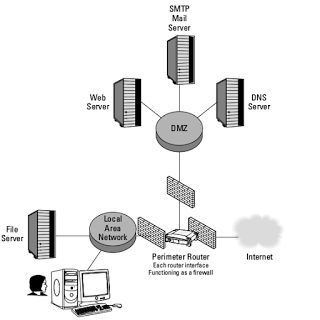
\includegraphics[width=0.70\textwidth]{figures/smtp.png}}
	\caption{SMTP}
	\label{smtp.png}
\end{figure}

\textbf{Skema Singkat}\par \vspace{12pt}
Mail Server atau yang sering disebut juga E-Mail server, digunakan untuk mengirim surat melalui Internet. Dengan begitu, dapat mempermudah dalam penggunanya, karena lebih cepat dan efisien. Untuk membuat Mail Server, harus terdapat SMTP dan POP3 server, yang digunakan untuk mengirim dan menerima email. Proses pengiriman email bisa terjadi karena adanya SMTP Server (Simple Mail Transfer Protocol). Setelah dikirim, email tersebut akan ditampung sementara di POP3 Server (Post Office Protocol ver. 3). Dan ketika user yang mempunyai email account tersebut online, mail client akan secara otomatis melakukan sinkronisasi dari POP3 Server.
\par \vspace{12pt}
Mungkin kita dulu pernah bahkan sering menggunakan kantor pos sebagai jasa untuk mengirim surat kepada kerabat atau teman kita yang jauh dari tempat kita tinggal, di Kantor pos itu juga terdapat Kurir sebagai tukang mengantarkan surat dari Kantor Pos kepada penerima.
\par \vspace{12pt}
SMTP ini singkatan dengan kepanjangan Simple Mail Transfer Protocol. Dengan pengertian singkat SMTP adalah protokol yang mengatur pengiriman email dari pengirim (Ongoing).
Cara kerja SMTP ini sama dengan Kantor Pos, tempat dimana kita menitipkan surat kita agar dikirimkan kepada penerima yang tertera di surat tersebut.
Terdapat pada port berapa SMTP? SMTP terdapat pada port 25.
\par \vspace{12pt}
POP3 ini singkatan dari kepanjangan Post Office Protocol ver.3 dan IMAP ini singkatan dari kepanjangan Internet Message Access Protocol. Dengan pengertian singkat POP3/IMAP adalah protokol yang mengatur penerimaan email kepada penerima (Ingoing).\par \vspace{12pt}
Cara kerja POP3 dan IMAP sama dengan kurir yang mengantarkan surat, tugasnya menyampaikan surat yang sebelumnya sudah dititipkan di Kantor Pos (SMTP) kepada penerima surat.
Terdapat pada port berapa POP3? POP3 terdapat pada port 110.
Terdapat pada port berapa IMAP? IMAP terdapat pada port 143.

Ada perbedaan antara POP3 dan IMAP, mudahnya. kalau IMAP itu protokol yang biasa kita pakai kalau kita pakai Web Based Mail, contohnya seperti (gmail.com, yahoo.com) dan menggunakan Browser sebagai antarmukanya, kalau POP3 menggunakan Aplikasi Email Client, sebut saja Outlook, Thunderbird, Outlook Express dll.

Bedanya jika kita pakai IMAP, kita hanya bisa melihat isi dari email yang ada pada mailbox kita secara online dan tidak bisa di download ke localdisk kita, berbeda dengan POP3 yang bisa membuka email secara offline dengan syarat ketika komputer online dia mendownload semua email ke local disk sehingga bisa dibaca offline.